%------------------------------------------------
%	PACKAGES AND THEMES
%------------------------------------------------

% this is a 4:3 layout.
\documentclass{beamer}
% for 16:9 use this command:
% \documentclass[aspectratio=169]{beamer}

\mode<presentation> {
\usetheme{metropolis}
\setbeamertemplate{caption}[numbered]
\setbeamertemplate{navigation symbols}{} % hide navigation symbols
}

\usepackage{graphicx} % images
\usepackage{algorithm2e}
\usepackage{mathtools}
\DeclarePairedDelimiter{\ceil}{\lceil}{\rceil}
\usepackage{algpseudocode}
\usepackage{booktabs} % allows the use of \toprule, \midrule and \bottomrule in tables
\usepackage[ngerman]{babel}
\usepackage[utf8]{inputenc}
\usepackage[T1]{fontenc}
\usepackage{mathtools}
\usepackage{xcolor}
\usepackage{listings} % code
\usepackage{pgf,tikz} % drawing
\usepackage{pifont} % new symbols
\usepackage{hyperref} % pretty links
% \usepackage{algorithmicx}
% \usepackage{algpseudocode}
% \usepackage[linesnumbered,ruled]{algorithm2e}

% for code keywords within the text
\usepackage{xcolor}
\definecolor{light-gray}{gray}{0.95}
\newcommand{\code}[1]{\colorbox{light-gray}{\texttt{#1}}}

\usepackage{lmodern}
\usepackage{subcaption}
\usepackage{textcomp}
% \usepackage{array}
% \usepackage{longtable}
% \usepackage{verbatim}
%\usepackage{tabularx}
\captionsetup[figure]{font=footnotesize}

\usepackage{amsmath}
\usepackage{amssymb}
\usepackage{amsthm}
% \usepackage{comment}
% \usepackage{enumitem}
% \usepackage[binary-units=true]{siunitx}
% \usepackage{thmtools}
\usepackage{csquotes}
\usepackage{tikz}
\usepackage{float}
\usetikzlibrary{automata,positioning}

% color settings for links
\hypersetup{
    colorlinks=true,
    urlcolor=blue,
    linkcolor=black,
    citecolor=green!50!black
}

\definecolor{mygreen}{RGB}{1,135,1}

\newcommand{\cmark}{\ding{51}}  % checkmark
\newcommand{\xmark}{\ding{55}}  % xmark
\newcommand\scalemath[2]{\scalebox{#1}{\mbox{\ensuremath{\displaystyle #2}}}}

\newcommand{\specialcell}[2][c]{%
  \begin{tabular}[#1]{@{}c@{}}#2\end{tabular}}

\setbeamerfont{bibliography item}{size=\footnotesize}
\setbeamerfont{bibliography entry author}{size=\footnotesize}
\setbeamerfont{bibliography entry title}{size=\footnotesize}
\setbeamerfont{bibliography entry location}{size=\footnotesize}
\setbeamerfont{bibliography entry note}{size=\footnotesize}

% \useoutertheme{miniframes} % navigation design
\useinnertheme{circles} % use non shiny circles (itemize, etc.)

% Main slide colors
% dunkel, hell, mittel
% \definecolor{pale}{RGB}{232, 236, 237}
% \definecolor{prim}{RGB}{53, 109, 120}
% \definecolor{sec}{RGB}{104, 170, 183}
% \definecolor{tert}{RGB}{109, 155, 168}
% \definecolor{quat}{RGB}{9, 59, 68}

\definecolor{pale}{RGB}{255, 255, 255}
% \definecolor{prim}{RGB}{153, 194, 173}
% good: \definecolor{prim}{RGB}{27, 33, 42}
\definecolor{prim}{RGB}{32, 43, 50}
\definecolor{sec}{RGB}{217, 232, 224}
\definecolor{tert}{RGB}{0, 82, 41}
% save
\definecolor{quat}{RGB}{0, 82, 41}

\setbeamercolor{palette primary}{bg=prim,fg=pale}
\setbeamercolor{palette secondary}{bg=sec,fg=pale}
\setbeamercolor{palette tertiary}{bg=tert,fg=pale}
\setbeamercolor{palette quaternary}{bg=quat,fg=pale}
\setbeamercolor{structure}{fg=prim} % itemize, enumerate, etc
\setbeamercolor{section in toc}{fg=prim} % TOC sections

% Block colors
\definecolor{example_color}{RGB}{93, 137, 98}
\definecolor{alert_color}{RGB}{175, 79, 72}

\setbeamercolor{normal text}{fg=prim!20!black,bg=pale!25!white}
\setbeamercolor{alerted text}{fg=alert_color!25!black}
\setbeamercolor{example text}{fg=example_color!25!black}

\setbeamercolor{block title example}{fg=white,bg=example_color}
\setbeamercolor{block body example}{fg=black,bg=example_color!10!white}
\setbeamercolor{block title alerted}{fg=white,bg=alert_color}
\setbeamercolor{block body alerted}{fg=black,bg=alert_color!10!white}

% Override palette coloring
\setbeamercolor{subsection in head/foot}{bg=quat,fg=pale}

\setbeamertemplate{frametitle}{%
    \nointerlineskip%

    \begin{beamercolorbox}[wd=\paperwidth,ht=2.5ex,dp=1ex]{frametitle}
        \hspace*{1ex}\insertframetitle%
        \ifx\insertframesubtitle@empty\else%
        {~\tiny\textcolor{quat!35!black}{\insertframesubtitle}}%
        \fi%
    \end{beamercolorbox}%
}

% math-command for bigger norm
\newcommand\norm[1]{\left\lVert#1\right\rVert}

% use this to include other files
% in this case style definitions for code
% alternative: \include{dateiname}
\lstdefinestyle{latex}{
    language=[LaTeX]TeX,
    inputencoding=utf8,
    basicstyle=\ttfamily,
    keywordstyle=\color{blue!60!black}, % use 60 percent blue and 40 black
    commentstyle=\color{cyan!60!black},
    tabsize=2,
    emph={document,itemize,enumerate,center,tabular,table,
    figure,wrapfigure,minipage,columns,align,bmatrix,
    lstlisting,beamer,frame,tikzpicture},
    emphstyle=\color{magenta!60!black},
    morekeywords={lstset,includegraphics,theenumi,labelitemi,column,color,url,href}
}

\lstdefinestyle{inline_latex}{
    language=[LaTeX]TeX,
    inputencoding=utf8,
    basicstyle=\ttfamily,
    resetmargins= true,
    belowcaptionskip=0pt,
    aboveskip=0pt,
    belowskip=0pt,
    keywordstyle=\color{blue!60!black},
    commentstyle=\color{cyan!60!black},
    emph={document,itemize,enumerate,center,tabular,table,
    figure,wrapfigure,minipage,columns,align,bmatrix,
    lstlisting,beamer,frame,tikzpicture,Parameter},
    emphstyle=\color{magenta!60!black},
    morekeywords={lstset,includegraphics,theenumi,labelitemi,column,color,url,href,Befehlsname}
}

\lstdefinestyle{cpp}{
    language=C++,
    basicstyle=\ttfamily,
    keywordstyle=\color{blue!90!black},
    stringstyle=\color{magenta!60!black},
    commentstyle=\color{green!35!black},
    morecomment=[l][\color{gray!60!black}]{\#},
    tabsize=2
}

\lstdefinestyle{empty}{
    basicstyle=\rmfamily,
    keywordstyle=\bfseries,
    commentstyle=\color{black}\itshape
}

\lstset{style=latex}

%------------------------------------------------
%	TITLE PAGE
%------------------------------------------------

\selectlanguage{ngerman}
\title[]{Execution Monitoring for Long-Term Autonomous Plant Observation with a Mobile Robot}

\author{Tim Bohne}
\institute[]
{
\textit{AG Knowledge-Based Systems}\newline
\textit{DFKI Plan-Based Robot Control Group}
\medskip
}
\date{\today}

% make slide at the beginnig of each section
\AtBeginSection[]{
{\setbeamercolor{background canvas}{bg=white}}}

% where images are locatied
\graphicspath{{./images/}}

\begin{document}

\begin{frame}[plain] % plain slides dont have navigation bars etc.
\titlepage % Print the title page as the first slide
\end{frame}

\begin{frame}
\frametitle{Übersicht} % table of contents slide
\tableofcontents
\end{frame}

%------------------------------------------------
\section{Szenario}
%------------------------------------------------

\begin{frame}
  \frametitle{Szenario in der Simulation}
  \begin{figure}[H]
    \centering
    \begin{subfigure}[b]{0.49\textwidth}
      \centering
      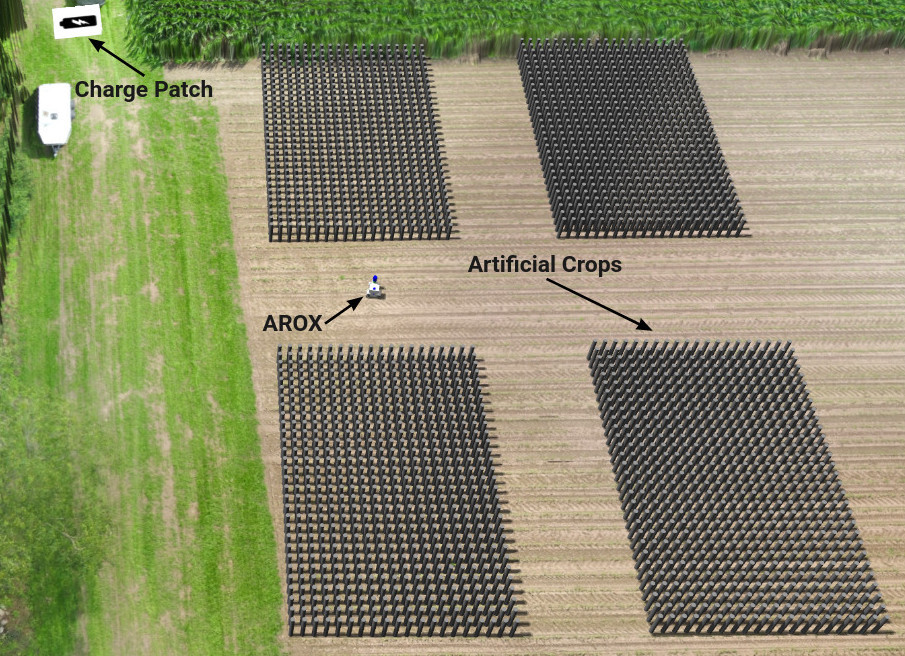
\includegraphics[width=\textwidth]{img/prototype_scenario.jpg}
      \caption*{\textsc{Prototypisches Layout}}
    \end{subfigure}
    \begin{subfigure}[b]{0.49\textwidth}
      \centering
      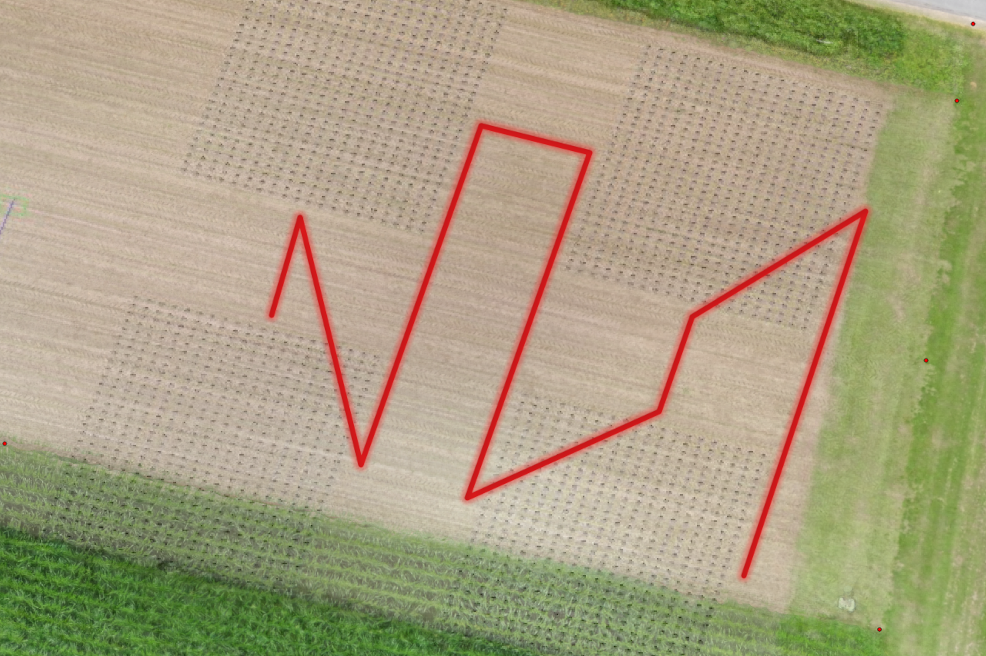
\includegraphics[width=\textwidth]{img/example_path.png}
      \caption*{\textsc{Beispiel-Scan-Route}}
    \end{subfigure}
  \end{figure}
  \begin{itemize}
    \item 3D-Lidar-Scans / Hyperspektralaufnahmen von Pflanzen \textrightarrow \thinspace \textbf{Wachstum überwachen / Merkmale erkennen}
    \item \textbf{Dynamische, unstrukturierte Umgebung}
    \item \textbf{$2.5D$-Simulation der Testfeld-Umgebung} in \textit{Gazebo} inkl. AROX-Modell (URDF)
  \end{itemize}
\end{frame}

%------------------------------------------------
\section{Langzeit-autonome mobile Roboter}
%------------------------------------------------

\begin{frame}
  \frametitle{Langzeit-autonome mobile Roboter}
  \textbf{Langfristigkeit}
  \begin{figure}[H]
    \centering
    \begin{subfigure}[b]{0.32\textwidth}
      \centering
      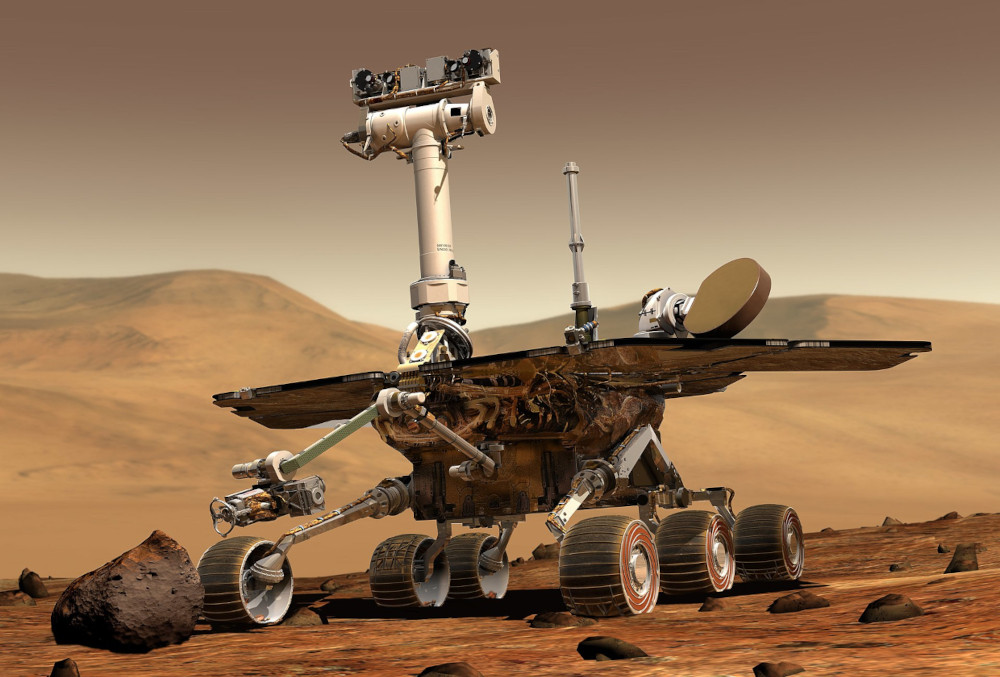
\includegraphics[width=\textwidth]{img/mars_rover.jpg}
      \caption*{\textsc{$\approx$ Jahre \cite{MarsRover}}}
    \end{subfigure}
    \begin{subfigure}[b]{0.32\textwidth}
      \centering
      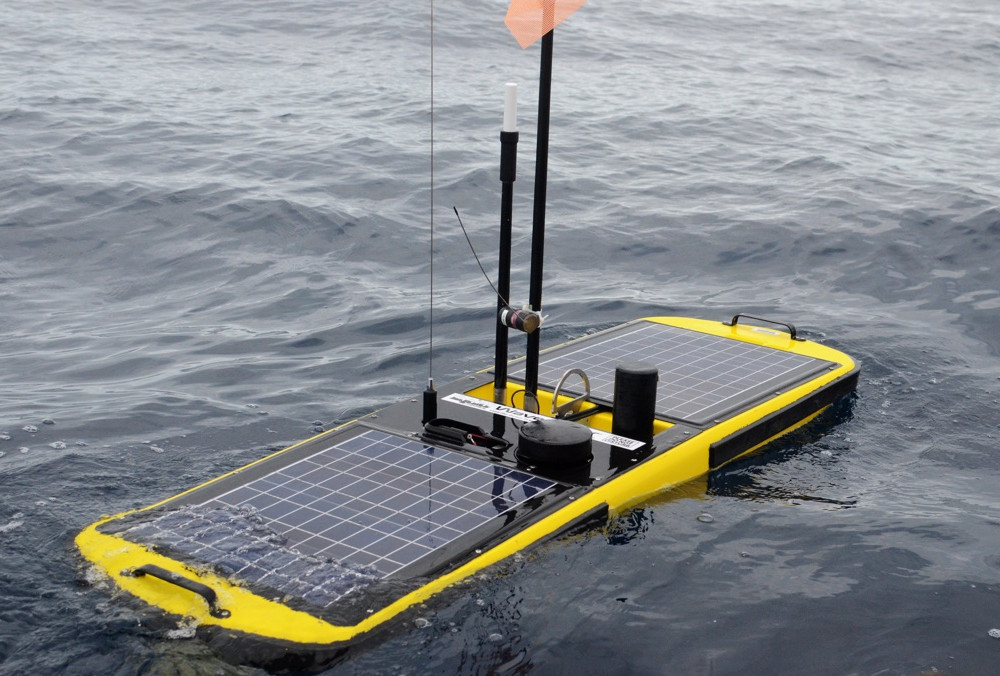
\includegraphics[width=\textwidth]{img/waveglider.jpg}
      \caption*{\textsc{$\approx$ Monate \cite{WaveGlider}}}
    \end{subfigure}
    \begin{subfigure}[b]{0.32\textwidth}
      \centering
      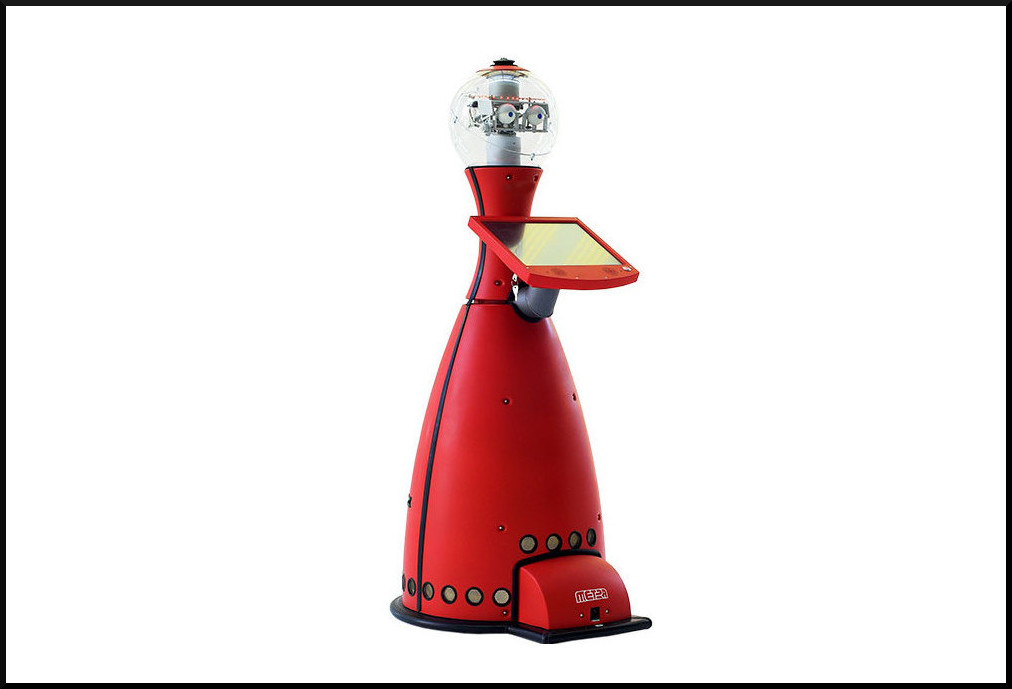
\includegraphics[width=\textwidth]{img/service_robot.jpg}
      \caption*{\textsc{$\approx$ Wochen \cite{ServiceRobot}}}
    \end{subfigure}
  \end{figure}
  \begin{itemize}
    \item Keine strikte Definition \textrightarrow \thinspace \textbf{kontextabhängig}
    \item \underline{Hier:}
    \begin{itemize}
      \item \textbf{Ladezyklus} - zeitlicher Handlungsradius des Roboters
      \item \textbf{Missionszyklus} - repetitiver Charakter der Mission
    \end{itemize}
    \item \textbf{LB}: Prozesse, die eine Reihe solcher Zyklen erfordern
    \item \textbf{UB}: Wartungsintervalle
  \end{itemize}
\end{frame}

\begin{frame}
  \frametitle{Langzeit-autonome mobile Roboter}
  \textbf{Autonomie}
  \begin{itemize}
    \item Ebenfalls nicht scharf definiert und \textbf{kontextabhängig}
    \item \textbf{Kooperation} nicht prinzipiell ausgeschlossen
    \item \underline{Hier:} \textbf{Vollautonom} - Inanspruchnahme menschlicher Hilfe ausschließlich im Fehlerfall
  \end{itemize}
  \begin{figure}[H]
    \centering
    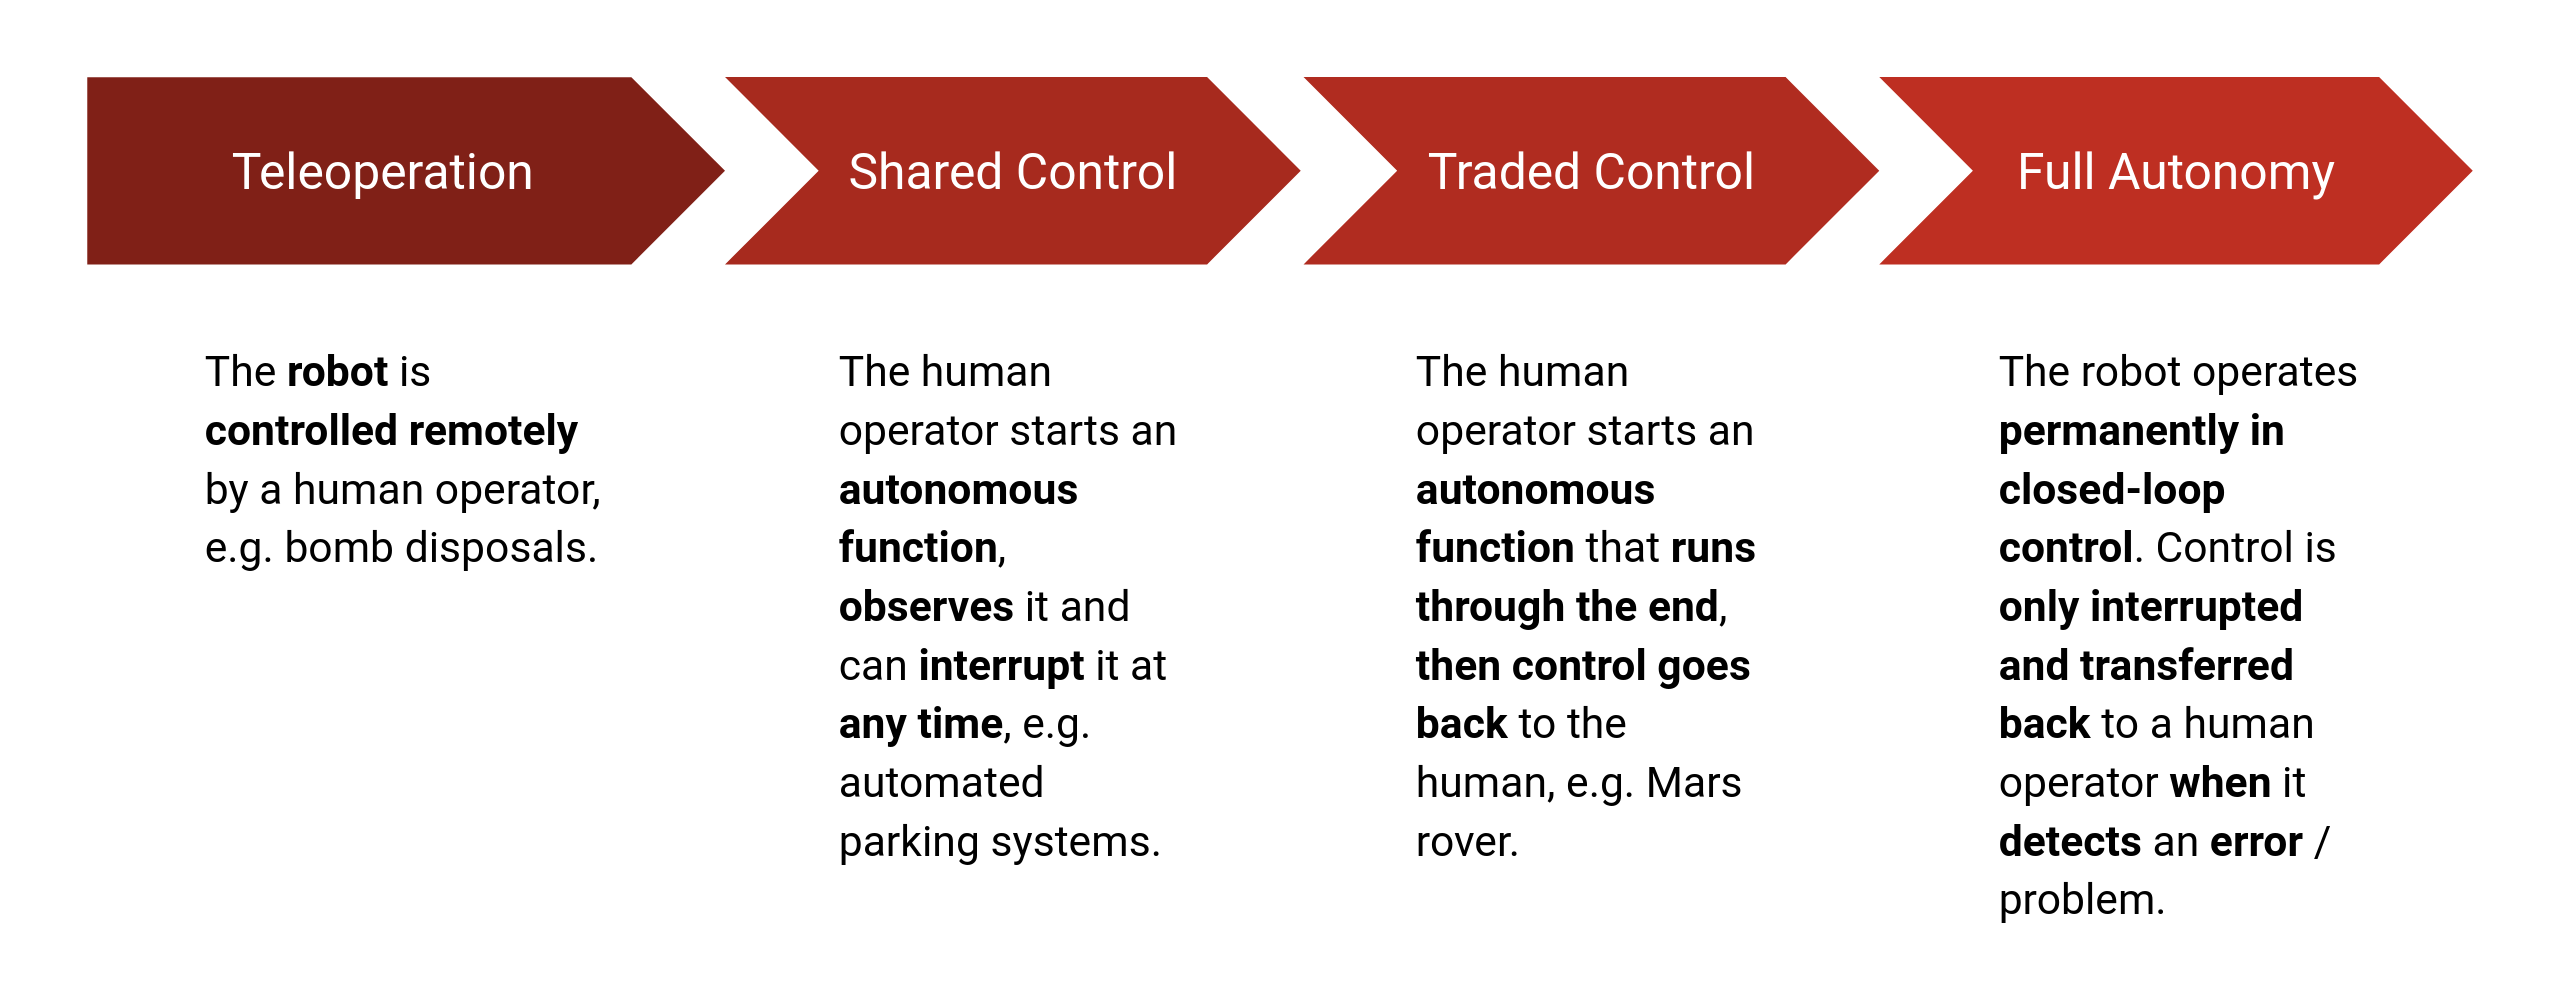
\includegraphics[width=\textwidth]{img/autonomy_spectrum.png}
    \caption*{\textsc{Spektrum der Autonomie (basierend auf \cite{Hertzberg:2015})}}
  \end{figure}
\end{frame}

\begin{frame}
  \frametitle{Langzeit-autonome mobile Roboter}
  \textbf{Mobilität}\newline
  System, das in der Lage ist, sich innerhalb bestimmter Grenzen frei in einer Umgebung zu bewegen \cite{Hertzberg:2012}
\end{frame}

\begin{frame}
  \frametitle{AROX - Autonomous Robotic Experimentation Platform}
  \begin{figure}[H]
    \centering
    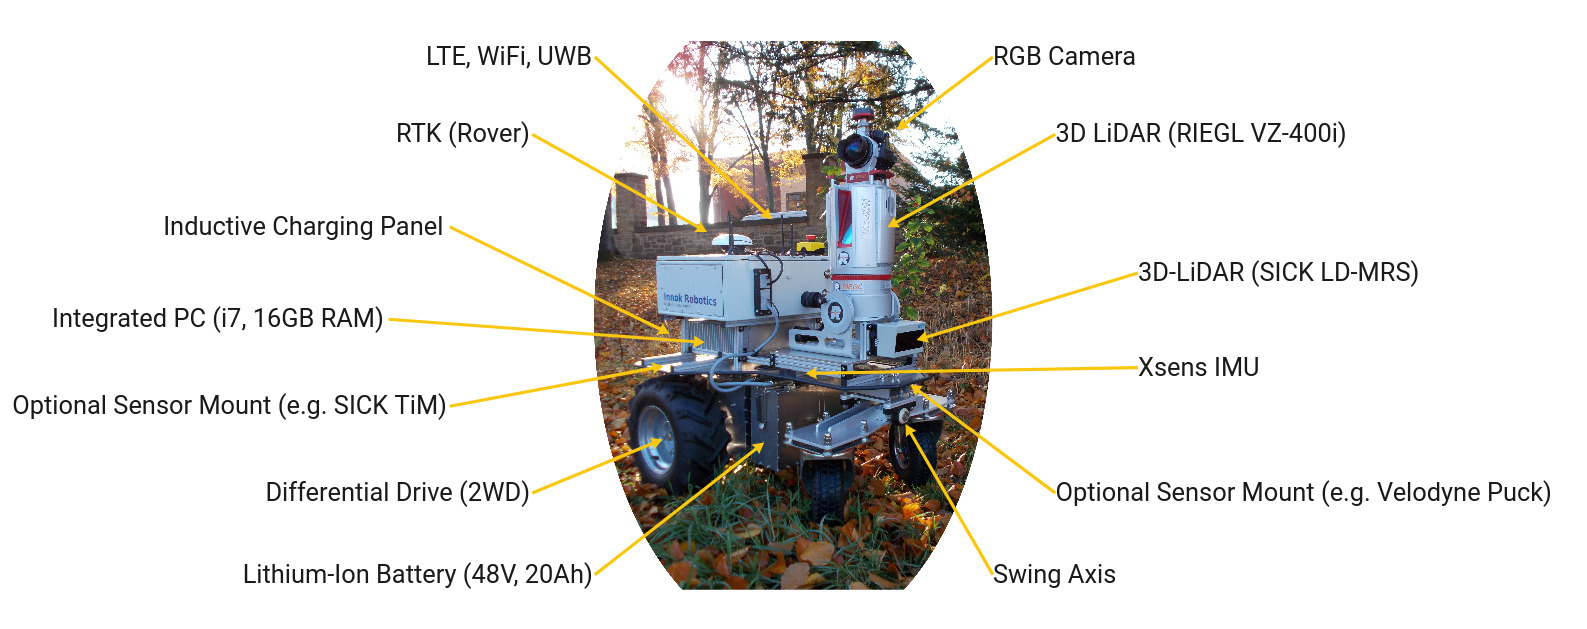
\includegraphics[width=\textwidth]{img/AROX.jpg}
  \end{figure}
  \textbf{Lokalisierung}: \code{robot\_localization} \cite{Moore:2014}\newline \textrightarrow \thinspace Sensorfusion von IMU-, Odometrie- und RTK-GNSS-Daten\newline
  \textbf{Navigation}: \code{move\_base\_flex} \cite{Puetz:2018}
\end{frame}

\begin{frame}
  \frametitle{Plangenerierung und -bereitstellung}
  \textbf{ROS-Service} parst manuell erstellte Pläne (CSV)\newline
  
  \textbf{Aktionsmenge}:\newline $\{$\code{drive\_to($lat$,$lng$,$\theta$)}, \code{return\_to\_base}, \code{charge}, \code{scan}$\}$\newline
  \textbf{Inkl. Container-Infrastruktur}: \code{dock}, \code{undock}
  \begin{figure}[H]
    \centering
    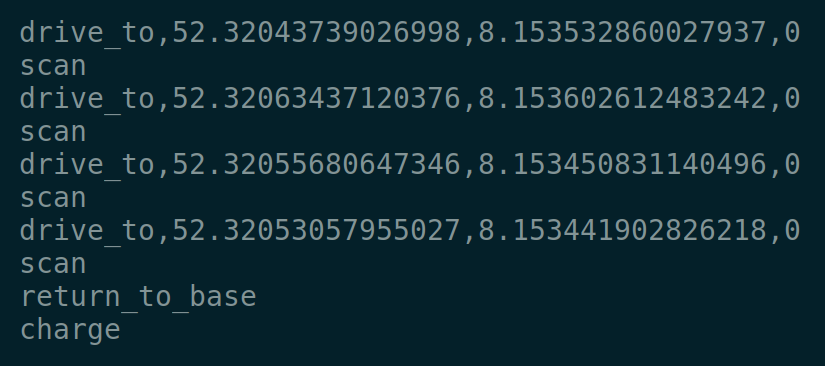
\includegraphics[width=0.85\textwidth]{img/plan_example.png}
    \caption*{\textsc{Beispielplan}}
  \end{figure}
\end{frame}

\begin{frame}
  \frametitle{Abstrakte Architektur autonomer Akteure}
  \begin{figure}[H]
    \centering
    \begin{subfigure}[b]{0.49\textwidth}
        \centering
        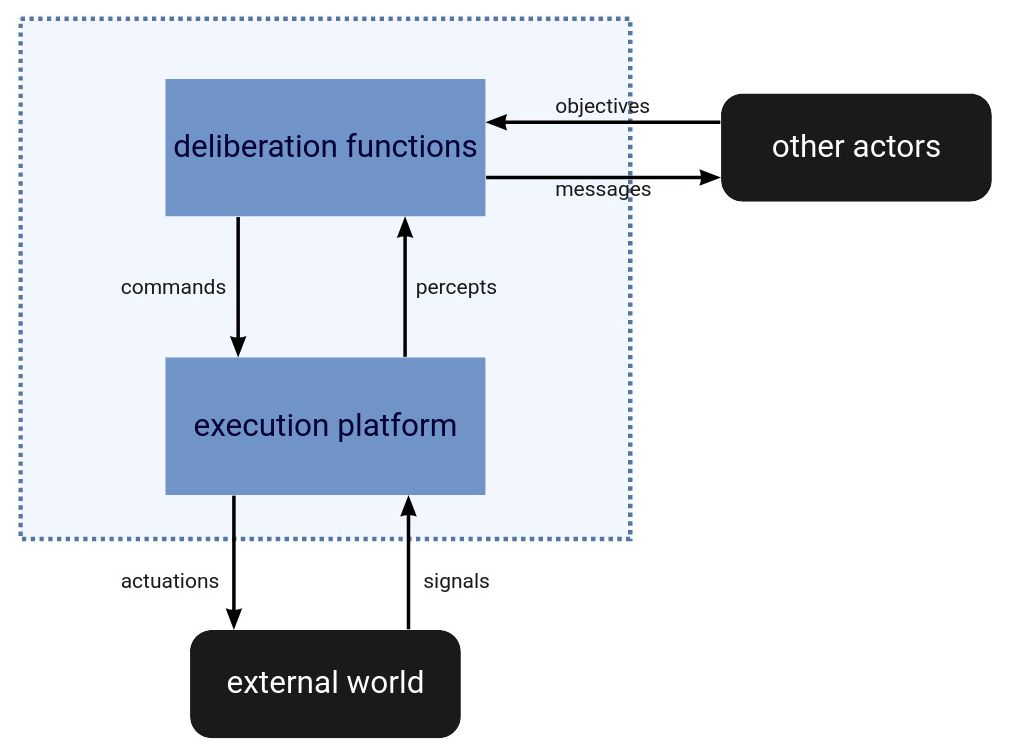
\includegraphics[width=\textwidth]{img/GNT_actor_new.png}
        \caption*{\textsc{\textquote{Actor} basierend auf GNT \cite{GNT:2016}}}
    \end{subfigure}
    \hfill
    \begin{subfigure}[b]{0.49\textwidth}
        \centering
        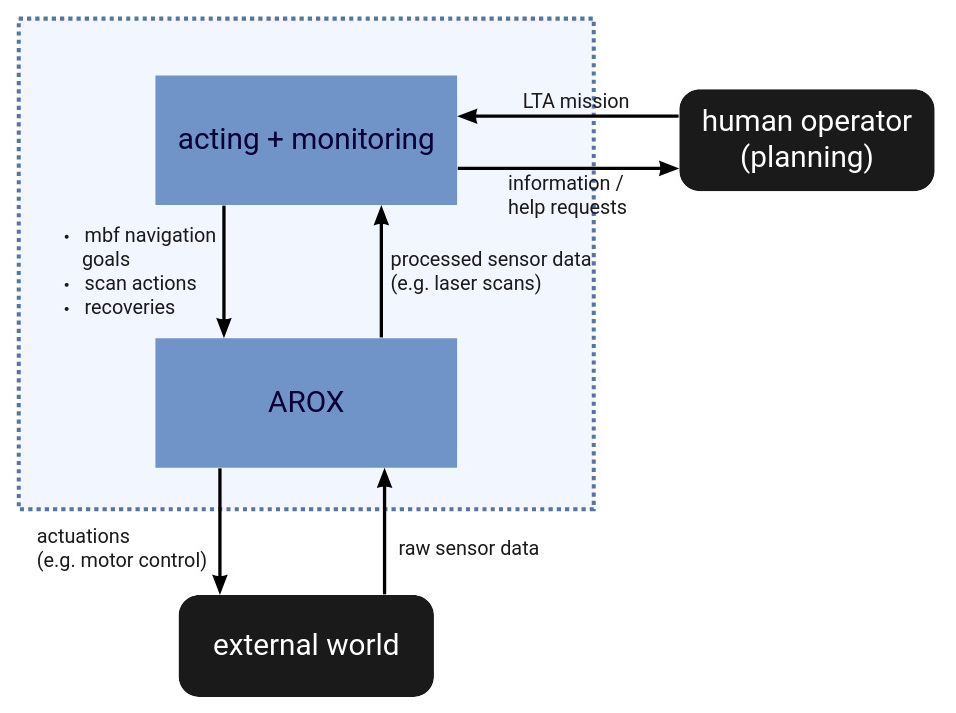
\includegraphics[width=\textwidth]{img/MSC_actor_new.png}
        \caption*{\textsc{Angewandt auf das betr. Szenario}}
    \end{subfigure}
  \end{figure}
\end{frame}

%------------------------------------------------
\section{Herausforderungen für Langzeitautonomie}
%------------------------------------------------

\begin{frame}
  \frametitle{Herausforderungen für Langzeitautonomie}
  \textbf{\underline{Bedingungen:}}
  \begin{enumerate}
    \item Kann im betrachteten Szenario \textbf{praktisch auftreten}
    \item Kann das reibungslose \textbf{Funktionieren des Systems} bzw. die \textbf{Qualität} der Ergebnisse \textbf{beeinträchtigen}
    \item Kann \textbf{durch Monitoring-Methoden detektiert} (gelöst / kommuniziert) werden
  \end{enumerate}
\end{frame}

\begin{frame}
  \frametitle{Herausforderungen für Langzeitautonomie}
  \begin{itemize}
    \item \textbf{Energiemanagement}
    \item \textbf{Fehlgeschlagener Ladevorgang}
    \item \textbf{Extreme Wetterbedingungen}
    \item \textbf{Sensorausfall (Wahrnehmung)}
    \item \textbf{Datenmanagement}
    \item \textbf{Verbindungsabbruch}
    \item \textbf{Navigationsfehler}
    \item \textbf{Fehlerhafte bzw. ungenaue Lokalisierung}
    \item \textbf{Planverteilungsfehler}
  \end{itemize}
  \textrightarrow \thinspace $48$ konkret behandelte Problemfälle\newline
  \textrightarrow \thinspace Viele weitere implizit abgedeckt
  % \begin{figure}[H]
  %   \raggedleft
  %   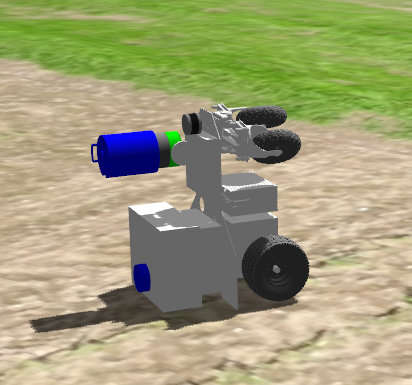
\includegraphics[width=0.3\textwidth]{img/AROX_fall.png}
  % \end{figure}
\end{frame}

\begin{frame}
  \frametitle{Herausforderungen für Langzeitautonomie}
  \textbf{\underline{Klassifikation:}}
  \begin{enumerate}
    \item Roboter detektiert ein Problem und ist in der Lage, es selbstständig zu lösen
    \item Roboter detektiert ein Problem, ist jedoch nicht in der Lage, es zu lösen \textrightarrow \thinspace informiert (menschlichen) Operator
    \item Roboter hat Störung / Problem, detektiert es jedoch nicht und kann es entsprechend weder lösen noch kommunizieren
  \end{enumerate}
  \textrightarrow \thinspace \textbf{Initial wird jedes potenzielle Problem als Typ $(3)$ eingestuft}\newline
  \textbf{Ziel}: Sämtliche Probleme in Kategorie $(1)$ / $(2)$ verschieben
\end{frame}

%------------------------------------------------
\section{Ausführungsüberwachung}
%------------------------------------------------

\begin{frame}
  \frametitle{Execution Monitoring State Machine}
  \textbf{High-Level Architektur der hierarchischen \textquote{State Machine} (ROS-SMACH)}
  \begin{figure}[H]
    \centering
    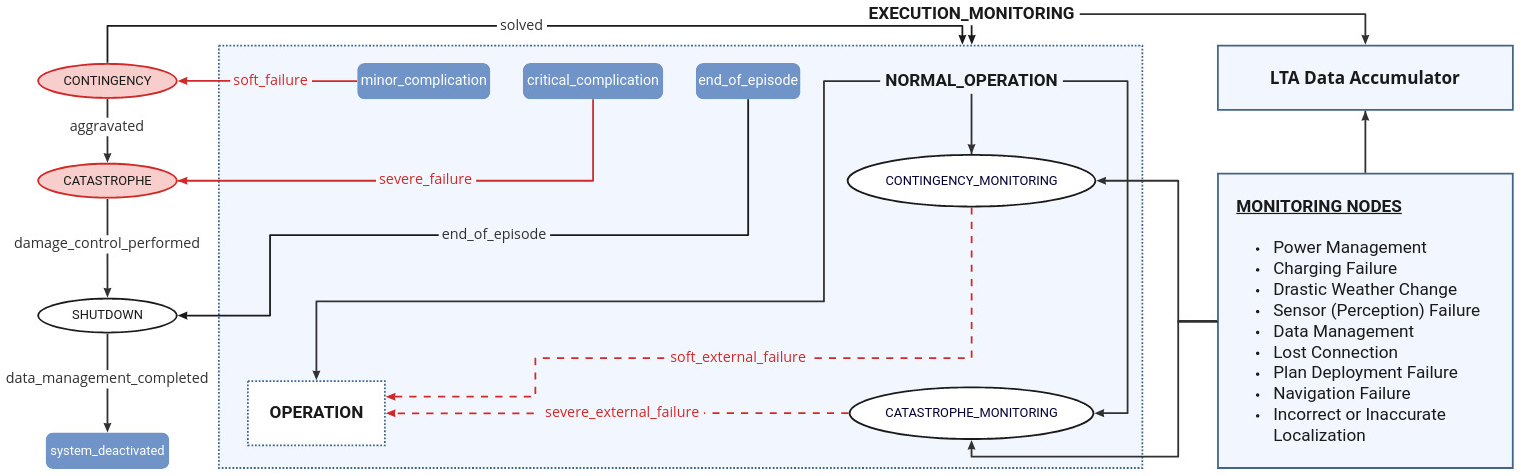
\includegraphics[width=\textwidth]{img/SMACH_high_level.png}
  \end{figure}
\end{frame}

\begin{frame}
  \frametitle{Execution Monitoring State Machine}
  \textbf{Architektur der eingebetteten \textquote{State Machine}}
  \begin{figure}[H]
    \centering
    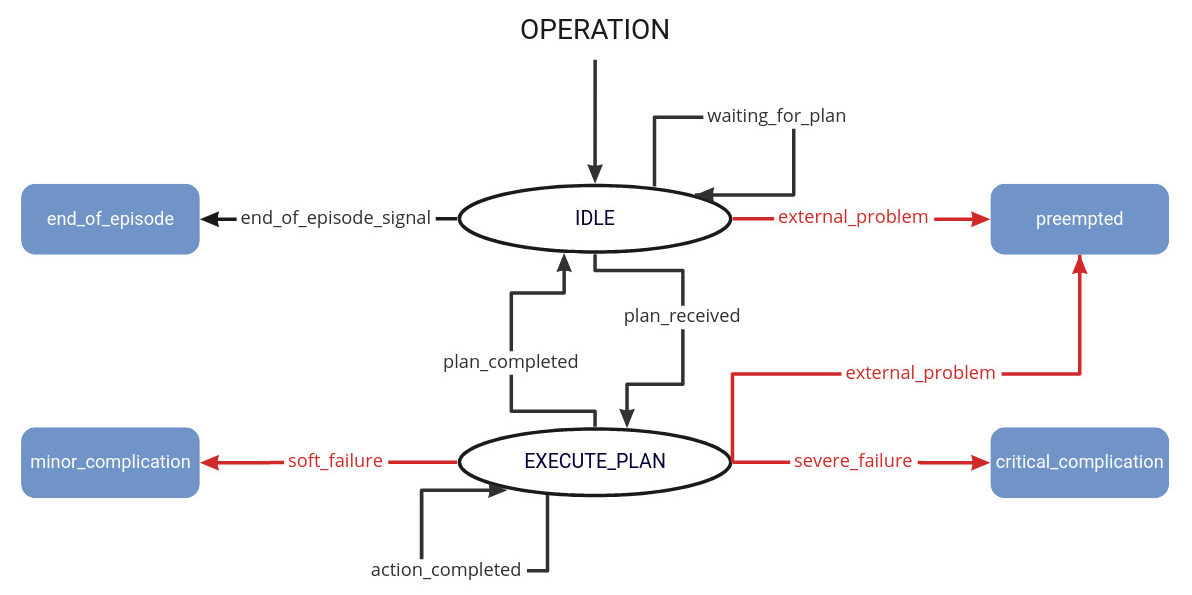
\includegraphics[width=0.8\textwidth]{img/SMACH_low_level.png}
  \end{figure}
\end{frame}

\begin{frame}
  \frametitle{Unterbrechung und Wiederaufnahme des normalen Betriebs}
  \underline{\textbf{Zwei Fälle:}}
  \begin{enumerate}
    \item \code{IDLE} \textrightarrow \thinspace trivial
    \item \code{EXECUTE\_PLAN} \textrightarrow \thinspace Plan $\pi$ im \code{userdata}-Feld des Zustands gespeichert
    \begin{itemize}
      \item Aktion $a \in \pi$ erfolgreich ausgeführt\newline \textrightarrow \thinspace $\pi := \pi \backslash \{a\}$ Input der nächsten Iteration
      \item Problem \textrightarrow \thinspace Unterbrechung der Planausführung
      \item Problem gelöst \textrightarrow \thinspace \code{IDLE} 
      \begin{itemize}
        \item $\pi \in \code{userdata.input\_plan}, \pi \neq \emptyset$ \textrightarrow \thinspace \textbf{Plan $\pi$ fortsetzen}
        \item $\code{userdata.input\_plan} = \emptyset$ \textrightarrow \thinspace \textbf{Neuen Plan anfordern}
      \end{itemize}
    \end{itemize}
  \end{enumerate}
\end{frame}

\begin{frame}
  \frametitle{Unterbrechung und Wiederaufnahme des normalen Betriebs}
  \underline{\textbf{Planausführung fortsetzen}}
  \begin{itemize}
    \item Geplante Ladestopps nicht notwendigerweise weiterhin zulässig
    \item \textbf{Unterbrechung mit Rückkehr zur Basis-Station} \textrightarrow \thinspace Planausführung \textbf{zulässig}
    \item \textbf{Unterbrechung ohne Rückkehr zur Basis-Station} \textrightarrow \thinspace Roboter verbraucht ungeplante Ressourcen, sodass a priori Ladestopp-Planung
    \textbf{unzulässig} wird \textrightarrow \thinspace Batterie-Monitoring
  \end{itemize}
\end{frame}

\begin{frame}
  \frametitle{Exemplarisch: GNSS-Verbindungsprobleme}
  \definecolor{myred}{rgb}{0.95,0.29,0.18}
  \definecolor{myblue}{rgb}{0.28,0.31,0.71}
  \begin{figure}[H]
    \centering
    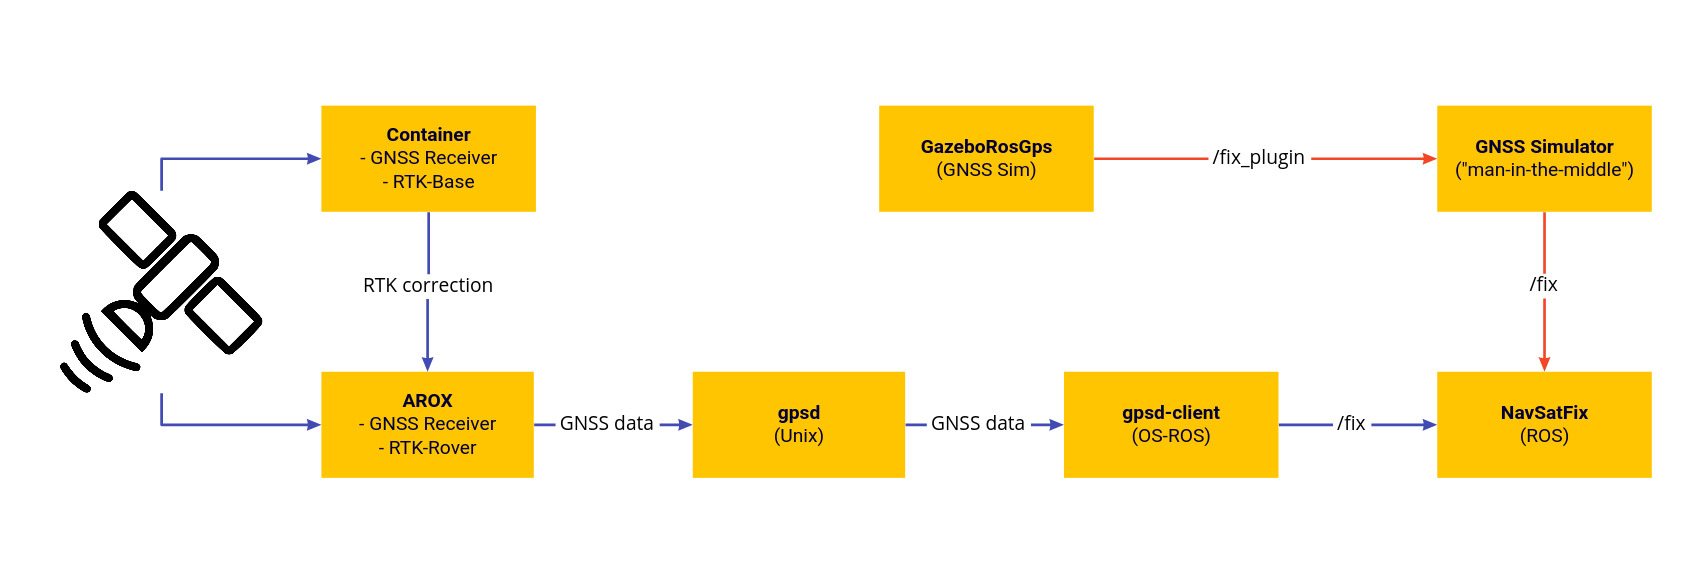
\includegraphics[width=\textwidth]{img/GNSS_comm.png}
  \end{figure}
  \textbf{\textcolor{myblue}{Praxis}} / \textbf{\textcolor{myred}{Simulation}}\linebreak
  \textbf{Resultat:} \code{NavSatFix}-Daten auf \code{/fix}-Topic
\end{frame}

\begin{frame}
  \frametitle{Exemplarisch: GNSS-Verbindungsprobleme}
  \begin{figure}[H]
    \centering
    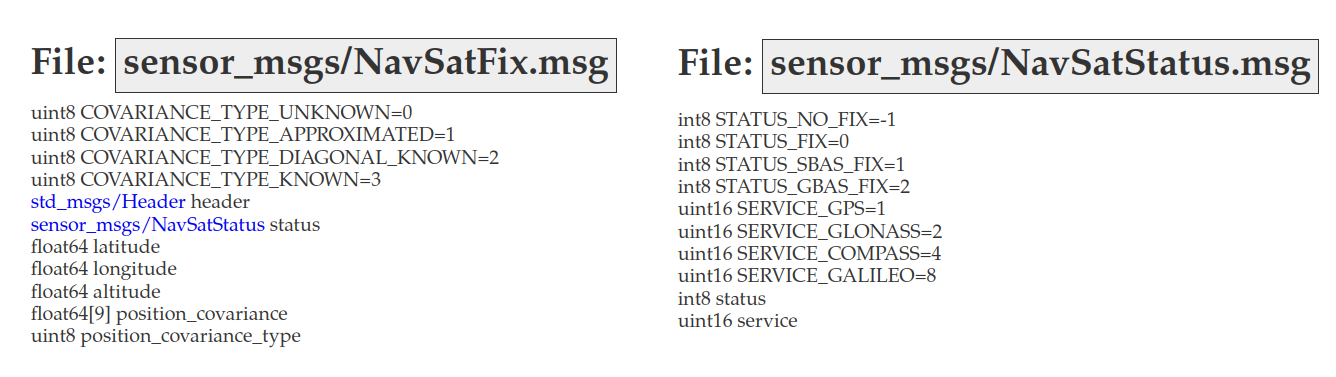
\includegraphics[width=\textwidth]{img/navsatfix.png}
  \end{figure}
  \textbf{Kovarianzmatrix}: $c_{ij} \in C_{3 \times 3}$, $i, j \in \{E, N, U\}$

  \textbf{Standardabweichung ($m$)}: $\sqrt{c_{ii}} \thinspace \forall \thinspace i \in \{E, N, U\}$
\end{frame}

\begin{frame}
  \frametitle{Exemplarisch: GNSS-Verbindungsprobleme}
  \begin{figure}[H]
    \centering
    \begin{subfigure}[b]{0.49\textwidth}
        \centering
        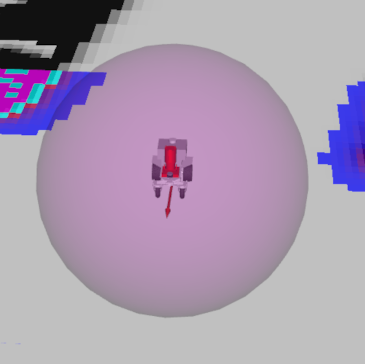
\includegraphics[width=0.75\textwidth]{img/GNSS_cov_low.png}
        \caption{\textsc{Relativ geringe Unsicherheit}}
    \end{subfigure}
    \hfill
    \begin{subfigure}[b]{0.49\textwidth}
        \centering
        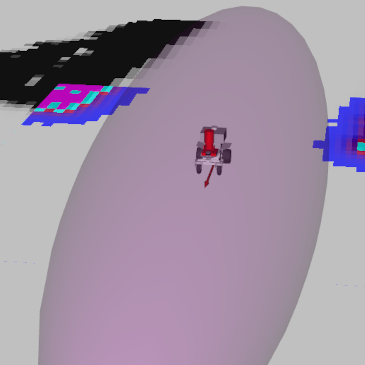
\includegraphics[width=0.75\textwidth]{img/GNSS_cov_high.png}
        \caption{\textsc{Hohe Unsicherheit bzgl.} $E$}
    \end{subfigure}
  \end{figure}
  \centering
  (a): $(\sqrt{6}m, \sqrt{6}m, \sqrt{6}m)$\linebreak
  (b): $(\sqrt{101}m, \sqrt{6}m, \sqrt{6}m)$\linebreak
  \textbf{Beide nicht ideal - kein RTK!}
\end{frame}

\begin{frame}
  \frametitle{Exemplarisch: GNSS-Verbindungsprobleme}
  \textbf{Qualitative Bewertung einer prinzipiell funktionierenden GNSS-Verbindung}
  \begin{itemize}
    \item \underline{\textbf{Hoch:}}
    \begin{itemize}
      \item \code{STATUS\_GBAS\_FIX}
      \item $\geq$ \code{COVARIANCE\_TYPE\_DIAGONAL\_KNOWN}
      \item $\sqrt{c_{ii}} \leq d_{max} \thinspace \forall \thinspace i \in \{E, N, U\}$, $d_{max} \in \mathbb{R}_{0}^{+}$
    \end{itemize}
    \item \underline{\textbf{Passabel:}}
    \begin{itemize}
      \item $\geq$ \code{STATUS\_FIX}
      \item $\geq$ \code{COVARIANCE\_TYPE\_APPROXIMATED}
      \item Standardabweichungen $\leq d_{max}$
    \end{itemize}
    \item \underline{\textbf{Gering:}}
    \begin{itemize}
      \item $\geq$ \code{STATUS\_FIX}
      \item Kovarianztyp unbekannt
    \end{itemize}
  \end{itemize}
  \textbf{Information via} \code{/robot\_info}
\end{frame}

\begin{frame}
  \frametitle{Exemplarisch: GNSS-Verbindungsprobleme}
  \textbf{Problemfall: Nachricht auf \code{/contingency\_preemption}}
  \begin{itemize}
    \item Verbindungsabbruch (Topic-Check)
    \item Status unzulässig bzw. \code{STATUS\_NO\_FIX}
    \item Längen- und Breitengrad-Informationen nicht vorhanden bzw. unzulässig
    \item Unsicherheit - Standardabweichungen
    \begin{itemize}
      \item Absolute Werte ($\leq d_{max}$)
      \item Entwicklung über die Zeit
    \end{itemize}
  \end{itemize}
  \textbf{Lösung}: Kurze Auszeit \textrightarrow \thinspace Erneuter Verbindungstest \textrightarrow \thinspace Kommunikation des Problems bei wiederholtem Misserfolg

  \textbf{Kompatibel mit sämtlichen Systemen, die \code{NavSatFix} verwenden!}
\end{frame}

% \begin{frame}
%   \frametitle{Exemplarisch: Navigationsfehler}
%   \textbf{Fall 1}: Es existiert ein Pfad, \code{move\_base\_flex} findet ihn jedoch nicht (direkt)
%   \begin{figure}[H]
%     \centering
%     \begin{subfigure}[b]{0.49\textwidth}
%         \centering
%         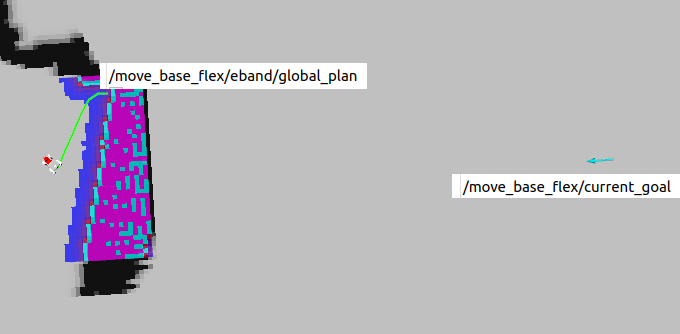
\includegraphics[width=\textwidth]{img/nav_fail_wrong_route_0.png}
%         \caption{\code{move\_base\_flex}\textsc{-Route (rviz)}}
%         \label{fig:nav_fail_rviz}
%     \end{subfigure}
%     \hfill
%     \begin{subfigure}[b]{0.49\textwidth}
%         \centering
%         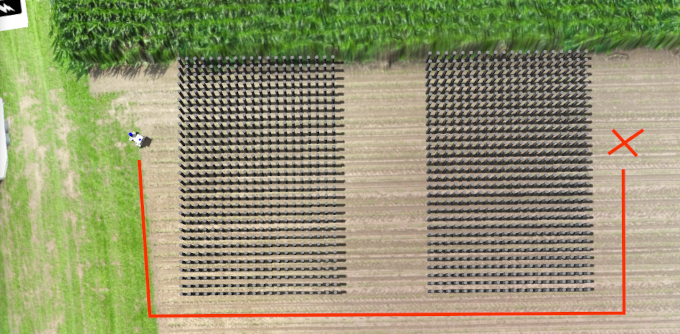
\includegraphics[width=\textwidth]{img/nav_fail_wrong_route_1.png}
%         \caption{\textsc{Zulässige Route (Gazebo)}}
%         \label{fig:nav_fail_gazebo}
%     \end{subfigure}
%   \end{figure}
%   \begin{itemize}
%     \item \textbf{\textquote{Sustained Recovery}} - nicht beliebig lange warten
%     \begin{itemize}
%       \item Übergänge zählen:\newline \code{GoalStatus.ACTIVE} \textrightarrow \thinspace \code{GoalStatus.ABORTED}
%       \item \code{GoalStatus.SUCCEEDED} setzt Zähler zurück
%       \item Position zu Beginn berücksichtigen (\code{/fix}) - Zielannäherung?
%     \end{itemize}
%     \item \textbf{Explizite \code{move\_base\_flex} Fehler}
%   \end{itemize}
% \end{frame}

% \begin{frame}
%   \frametitle{Exemplarisch: Navigationsfehler}
%   \textbf{Fall 2}: Es existiert kein Pfad
%   \begin{figure}[H]
%     \centering
%     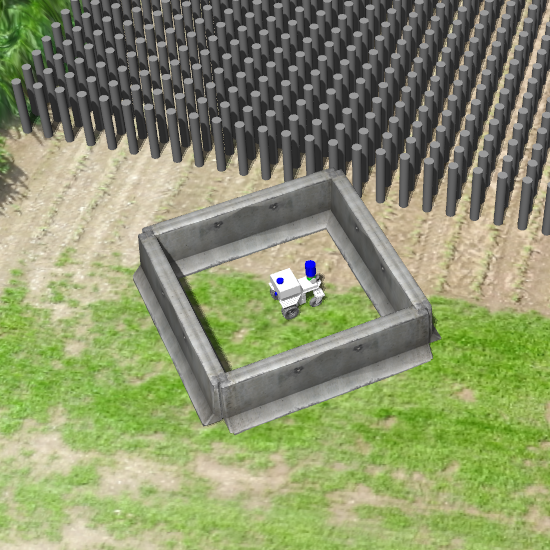
\includegraphics[width=0.3\textwidth]{img/robot_prison.png}
%     \caption*{\code{/spawn\_robot\_prison}}
%   \end{figure}
%   \begin{itemize}
%     \item Ebenfalls durch Monitoring für \textbf{\textquote{Sustained Recovery}} und \textbf{explizite \code{move\_base\_flex} Fehler} abgedeckt
%     \item Endet in jedem Fall in \code{CATASTROPHE} - nicht lösbar
%   \end{itemize}
% \end{frame}

% \begin{frame}
%   \frametitle{Exemplarisch: Navigationsfehler}
%   \textbf{Lösungsversuch für Navigationsprobleme}
%   \begin{itemize}
%     \item Unabhängig von der Ursache (\textquote{Sustained Recovery} / \code{move\_base\_flex}-Fehler)
%     \item Einträge in den globalen und lokalen \textquote{Costmaps} löschen \textrightarrow \thinspace nicht mehr vorhandene Hindernisse entfernen
%     \item Roboter zu einem von mehreren konfigurierbaren, leicht zugänglichen Recorery-Punkten navigieren (missionsspezifisch)
%     \begin{itemize}
%       \item Befreit den Roboter häufig aus \textquote{Deadlock}-Situationen
%       \item Idee: Problem aus einer anderen Perspektive betrachten
%       \item Monitoring muss weiterhin stattfinden (vgl. \textquote{Robot Prison})
%     \end{itemize}
%   \end{itemize}
%   \textbf{Kompatibel mit sämtlichen Systemen, die \code{move\_base(\_flex)} verwenden!}
% \end{frame}

%------------------------------------------------
\section{Experimente / Evaluation}
%------------------------------------------------

\begin{frame}
  \frametitle{Experimente - Grundsätzliches Vorgehen}
  (\textbf{Problem-Simulation} \textrightarrow) \thinspace \textbf{Monitoring} \textrightarrow \thinspace \textbf{Lösung}
  \begin{itemize}
    \item \textbf{Simulation:} Auslösbar durch Nachricht auf Topic, z.B. \code{rostopic pub -1 /toggle\_snow\_sim std\_msgs/String fail}
    \item \textbf{Monitoring:} Detektiert Problem, unterbricht \code{NORMAL\_OPERATION}, initiiert geeignete Lösung
    \item \textbf{Lösung:}
    \begin{itemize}
      \item Problem gelöst \textrightarrow \thinspace Übergang zu \code{NORMAL\_OPERATION}
      \item Problem nicht gelöst \textrightarrow \thinspace Übergang zu \code{CATASTROPHE}
    \end{itemize}
  \end{itemize}
\end{frame}

\begin{frame}
  \frametitle{Experimente}
  \textbf{S1:} Zeigen, dass die Missionen \textbf{ohne Simulation eines der identifizierten Probleme} über einen längeren Zeitraum fehlerfrei läuft
  \begin{itemize}
    \item \textbf{Verifikation des Beispielplans}
    \item \textbf{Demonstration der grundsätzlichen Funktionalität}
  \end{itemize}
  \underline{\textbf{Def. gescheiterte Mission:}}
  \begin{enumerate}
    \item $> 900s$ keine Nachricht auf \code{arox/ongoing\_operation} trotz offener Tasks
    \item \code{hard\_failure} in \code{OPERATION} \textrightarrow \thinspace \code{CATASTROPHE}
  \end{enumerate}
  \textbf{$3$ Durchläufe á $4$ Stunden:}\newline
  \textrightarrow \thinspace \O $84$ Tasks, keine gescheiterte Mission
\end{frame}

\begin{frame}
  \frametitle{Experimente}
  \textbf{S2: Klassifikation der Problemkategorien in Bezug auf ihren potenziellen (worst-case) Schaden}
  \begin{figure}[H]
    \centering
    \resizebox{\textwidth}{!}{
    \begin{tabular}{| c | c | c | c | c |}
        \hline
        \textbf{problem} & \specialcell{\textbf{contingency} \\ \small{\textit{(no contingencies without monitoring)}} \\ sim + prac} & \specialcell{\textbf{catastrophe} \\ \small{\textit{((\cmark) \textrightarrow indirectly)}} \\ sim \quad\quad\quad\quad prac} & \specialcell{\textbf{potential to render mission worthless} \\ sim \quad\quad\quad\quad prac} \\ \hline
        power\_management & \cmark & \cmark \quad\quad\quad\quad\quad \cmark & \cmark \quad\quad\quad\quad\quad \cmark \\ \hline
        charging\_failure & \cmark & \cmark \quad\quad\quad\quad\quad \cmark & \cmark \quad\quad\quad\quad\quad \cmark \\ \hline
        drastic\_weather\_change & \cmark & \thinspace\thinspace \xmark \quad\quad\quad\quad\quad (\cmark) & \xmark \quad\quad\quad\quad\quad \cmark \\ \hline
        sensor\_failure & \cmark & \xmark \thinspace\thinspace\quad\quad\quad\quad\quad \xmark & \cmark \quad\quad\quad\quad\quad \cmark \\ \hline
        data\_management & \cmark & \xmark \thinspace\thinspace\quad\quad\quad\quad\quad \xmark & \cmark \quad\quad\quad\quad\quad \cmark \\ \hline
        lost\_connection & \cmark & (\cmark) \quad\quad\quad\quad (\cmark) & \cmark \quad\quad\quad\quad\quad \cmark \\ \hline
        plan\_deployment\_failure & \cmark & \cmark \quad\quad\quad\quad\quad \cmark & \cmark \quad\quad\quad\quad\quad \cmark \\ \hline
        navigation\_failure & \cmark & (\cmark) \quad\quad\quad\quad (\cmark) & \cmark \quad\quad\quad\quad\quad \cmark \\ \hline
        incorrect\_localization & \cmark & (\cmark) \quad\quad\quad\quad (\cmark) & \cmark \quad\quad\quad\quad\quad \cmark \\ \hline
    \end{tabular}}
  \end{figure}
  \underline{\textquote{catastrophe}-Spalte (ohne Monitoring):}
  \begin{itemize}
    \item \cmark \textrightarrow \thinspace \textbf{Scheitern der Mission sicher}
    \item (\cmark) \textrightarrow \thinspace \textbf{Scheitern der Mission möglich}
    \item \xmark \textrightarrow \thinspace \textbf{Wertlose Ergebnisse} (Ausnahme Extremwetter)
  \end{itemize}
\end{frame}

\begin{frame}
  \frametitle{Experimente}
  \textbf{S3: Evaluation der Monitoring-Ansätze}\newline
  $10$ Durchläufe á $5$ Stunden\newline
  Zufälliger Fehlerfall alle $250s$\newline
  \textbf{\underline{Betrachtete Aspekte:}}
  \begin{itemize}
    \item Erfolgreich abgeschlossene Mission
    \item \textbf{Erwartete Reaktionen} auf Fehlerfälle
    \begin{itemize}
      \item Korrekte \code{CONTINGENCY}-Situationen
      \item Korrekte \textquote{$\lnot$\code{CONTINGENCY}-Situationen}
    \end{itemize}
    \item \textbf{Unerwartete Reaktionen}
    \begin{itemize}
      \item Falsch-positiv / falsch-negativ
      \item Falsche Reaktion (Problemidentifikation)
    \end{itemize}
    \item Erfolgreich abgeschlossene Tasks
    \item Lade- und Missionszyklen
    \item Zurückgelegte Distanz
  \end{itemize}
\end{frame}

\begin{frame}
  \frametitle{Korrekte \textquote{$\lnot$\textsc{CONTINGENCY}-Situationen}}
  \textbf{Simulation statischer Hindernisse} (mit Ausweg)
  \begin{figure}[H]
    \centering
    \begin{subfigure}[b]{0.24\textwidth}
        \centering
        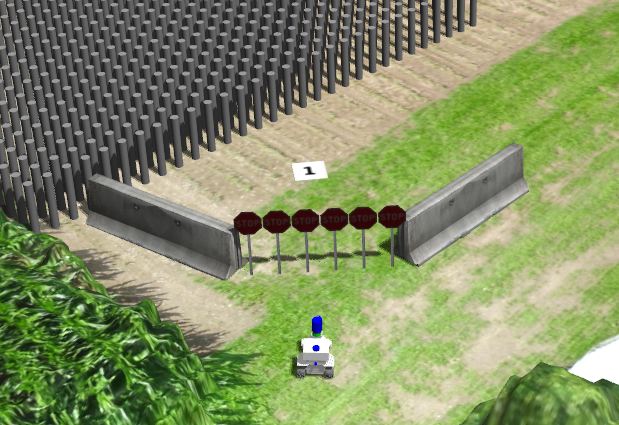
\includegraphics[width=\textwidth]{img/static_1.png}
        \caption{\textsc{Szenario $1$}}
        \label{fig:static_1}
    \end{subfigure}
    \hfill
    \begin{subfigure}[b]{0.24\textwidth}
        \centering
        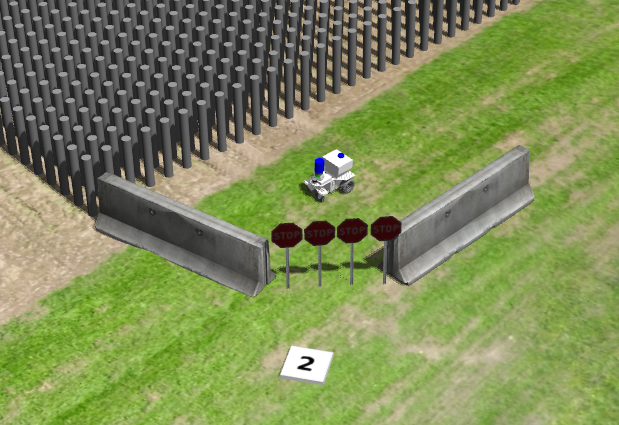
\includegraphics[width=\textwidth]{img/static_2.png}
        \caption{\textsc{Szenario $2$}}
        \label{fig:static_2}
    \end{subfigure}
    \begin{subfigure}[b]{0.24\textwidth}
        \centering
        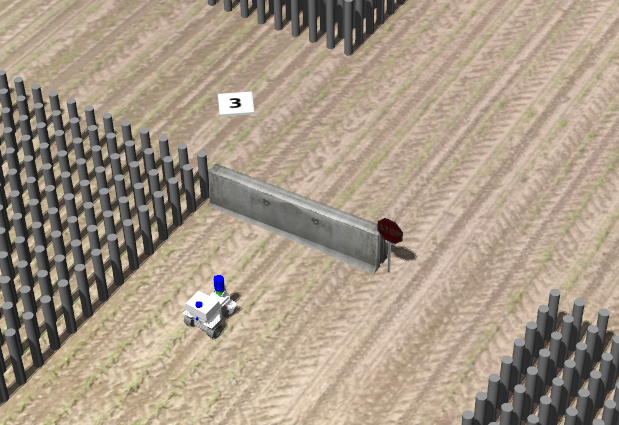
\includegraphics[width=\textwidth]{img/static_3.png}
        \caption{\textsc{Szenario $3$}}
        \label{fig:static_3}
    \end{subfigure}
    \hfill
    \begin{subfigure}[b]{0.24\textwidth}
        \centering
        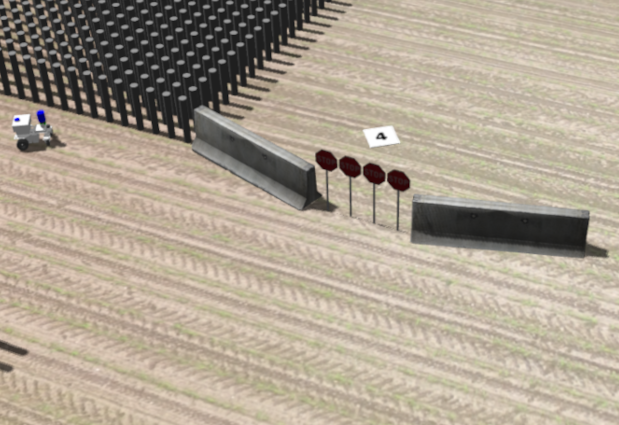
\includegraphics[width=\textwidth]{img/static_4.png}
        \caption{\textsc{Szenario $4$}}
        \label{fig:static_4}
    \end{subfigure}
  \end{figure}
  \newcommand{\squeezeup}{\vspace{-4.5mm}}
  \squeezeup
  \code{/spawn\_static\_obstacles} mit \code{msg} $scene_n$, $n \in \{1, 2, 3, 4\}$
  \begin{figure}[H]
    \centering
    \begin{subfigure}[b]{0.24\textwidth}
        \centering
        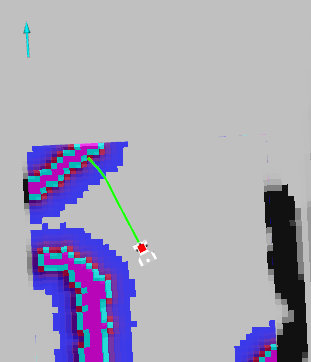
\includegraphics[width=\textwidth]{img/succ_1.png}
    \end{subfigure}
    \hfill
    \begin{subfigure}[b]{0.24\textwidth}
        \centering
        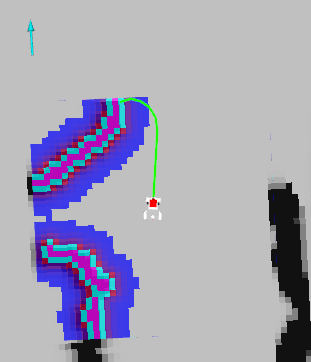
\includegraphics[width=\textwidth]{img/succ_2.png}
    \end{subfigure}
    \begin{subfigure}[b]{0.24\textwidth}
        \centering
        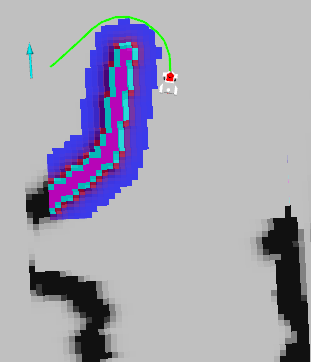
\includegraphics[width=\textwidth]{img/succ_3.png}
    \end{subfigure}
    \hfill
    \begin{subfigure}[b]{0.24\textwidth}
        \centering
        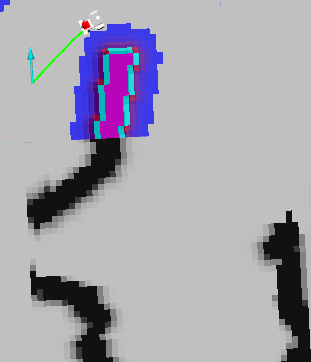
\includegraphics[width=\textwidth]{img/succ_4.png}
    \end{subfigure}
  \caption*{\textsc{Erfolgreiche Bewältigung von Szenario $1$}}
  \end{figure}
\end{frame}

% \begin{frame}
%   \frametitle{Fallback Solution - Requesting Help of a Human Operator}
% \end{frame}

\begin{frame}
  \frametitle{Ergebnisse}
  \begin{figure}[H]
    \centering
    \begin{subfigure}[b]{0.49\textwidth}
      \centering
      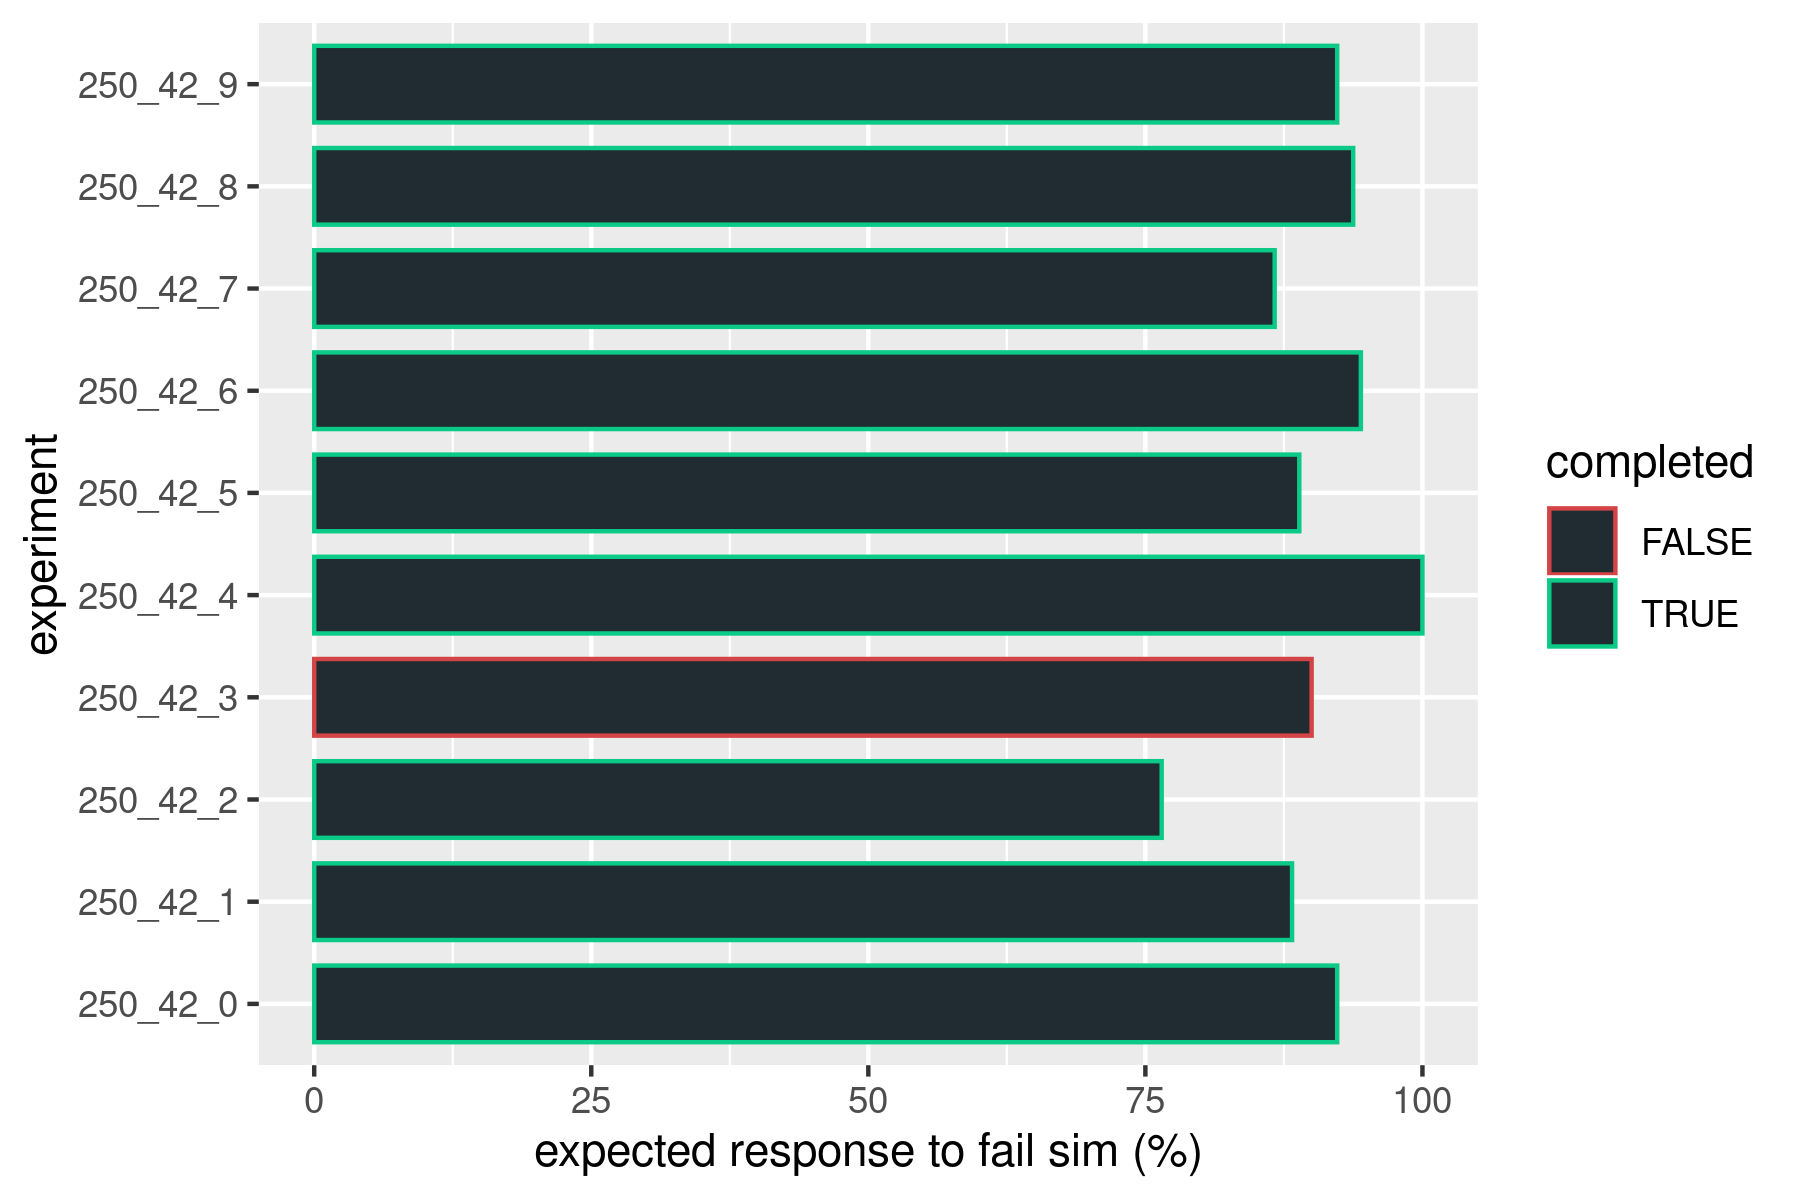
\includegraphics[width=\textwidth]{img/expected_res.png}
    \end{subfigure}
    \begin{subfigure}[b]{0.49\textwidth}
      \centering
      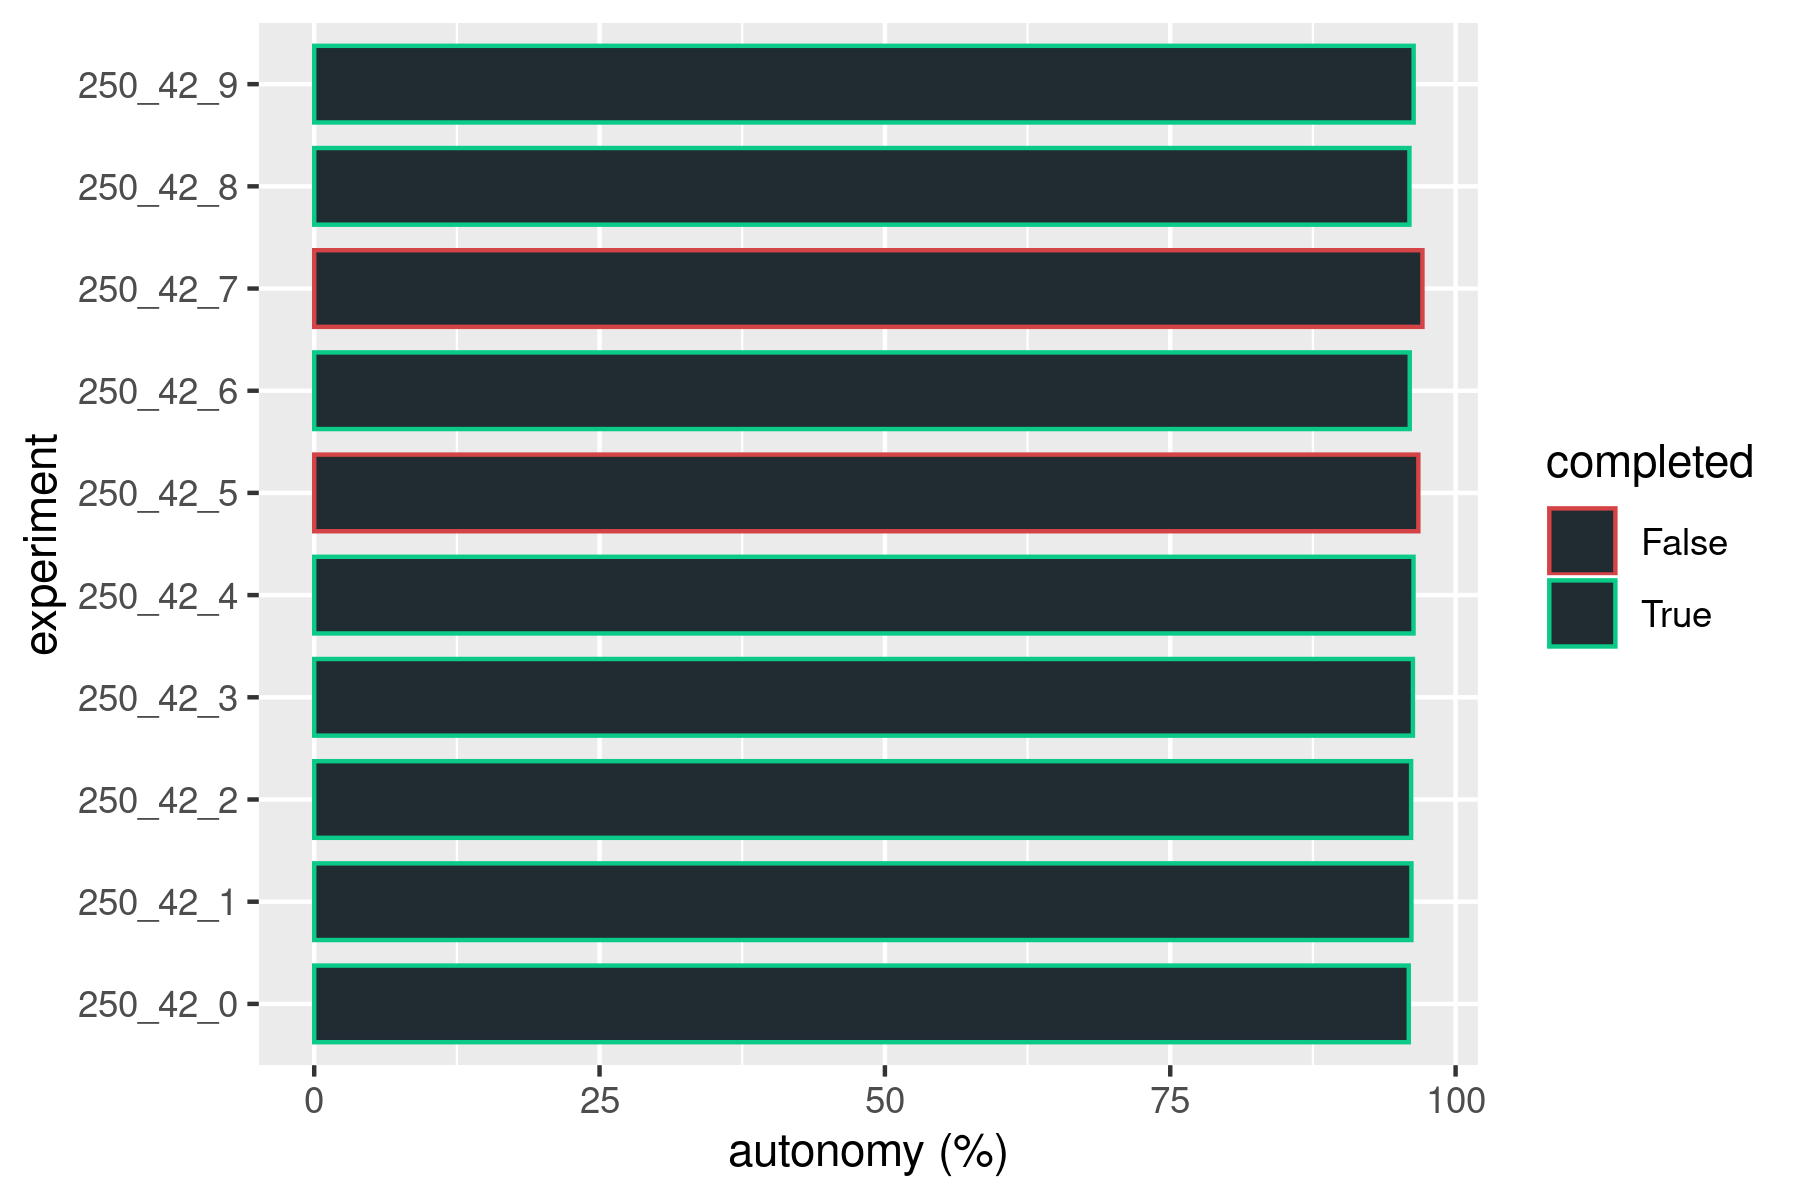
\includegraphics[width=\textwidth]{img/autonomy_percentage.png}
    \end{subfigure}
  \end{figure}
  \centering
  Laufzeit: \O $\thinspace \boldsymbol{3.85 h}$ / Ausgeführte Tasks: \O $\thinspace \boldsymbol{62.5}$\linebreak
  \centering
  Ladezyklen: \O $\thinspace \boldsymbol{7.3}$ / Missionszyklen: \O $\thinspace \boldsymbol{4.3}$\linebreak
  \centering
  Sim. Problemfälle: \O $\thinspace \boldsymbol{10}$ / Erwartete Reaktion: \O $\thinspace \boldsymbol{90.31 \%}$\linebreak
  \centering
  Zurückgelegte Distanz: \O $\thinspace \boldsymbol{1.4 km}$
\end{frame}

\begin{frame}
  \frametitle{Aktivitätsverteilung}
  \begin{figure}[H]
    \centering
    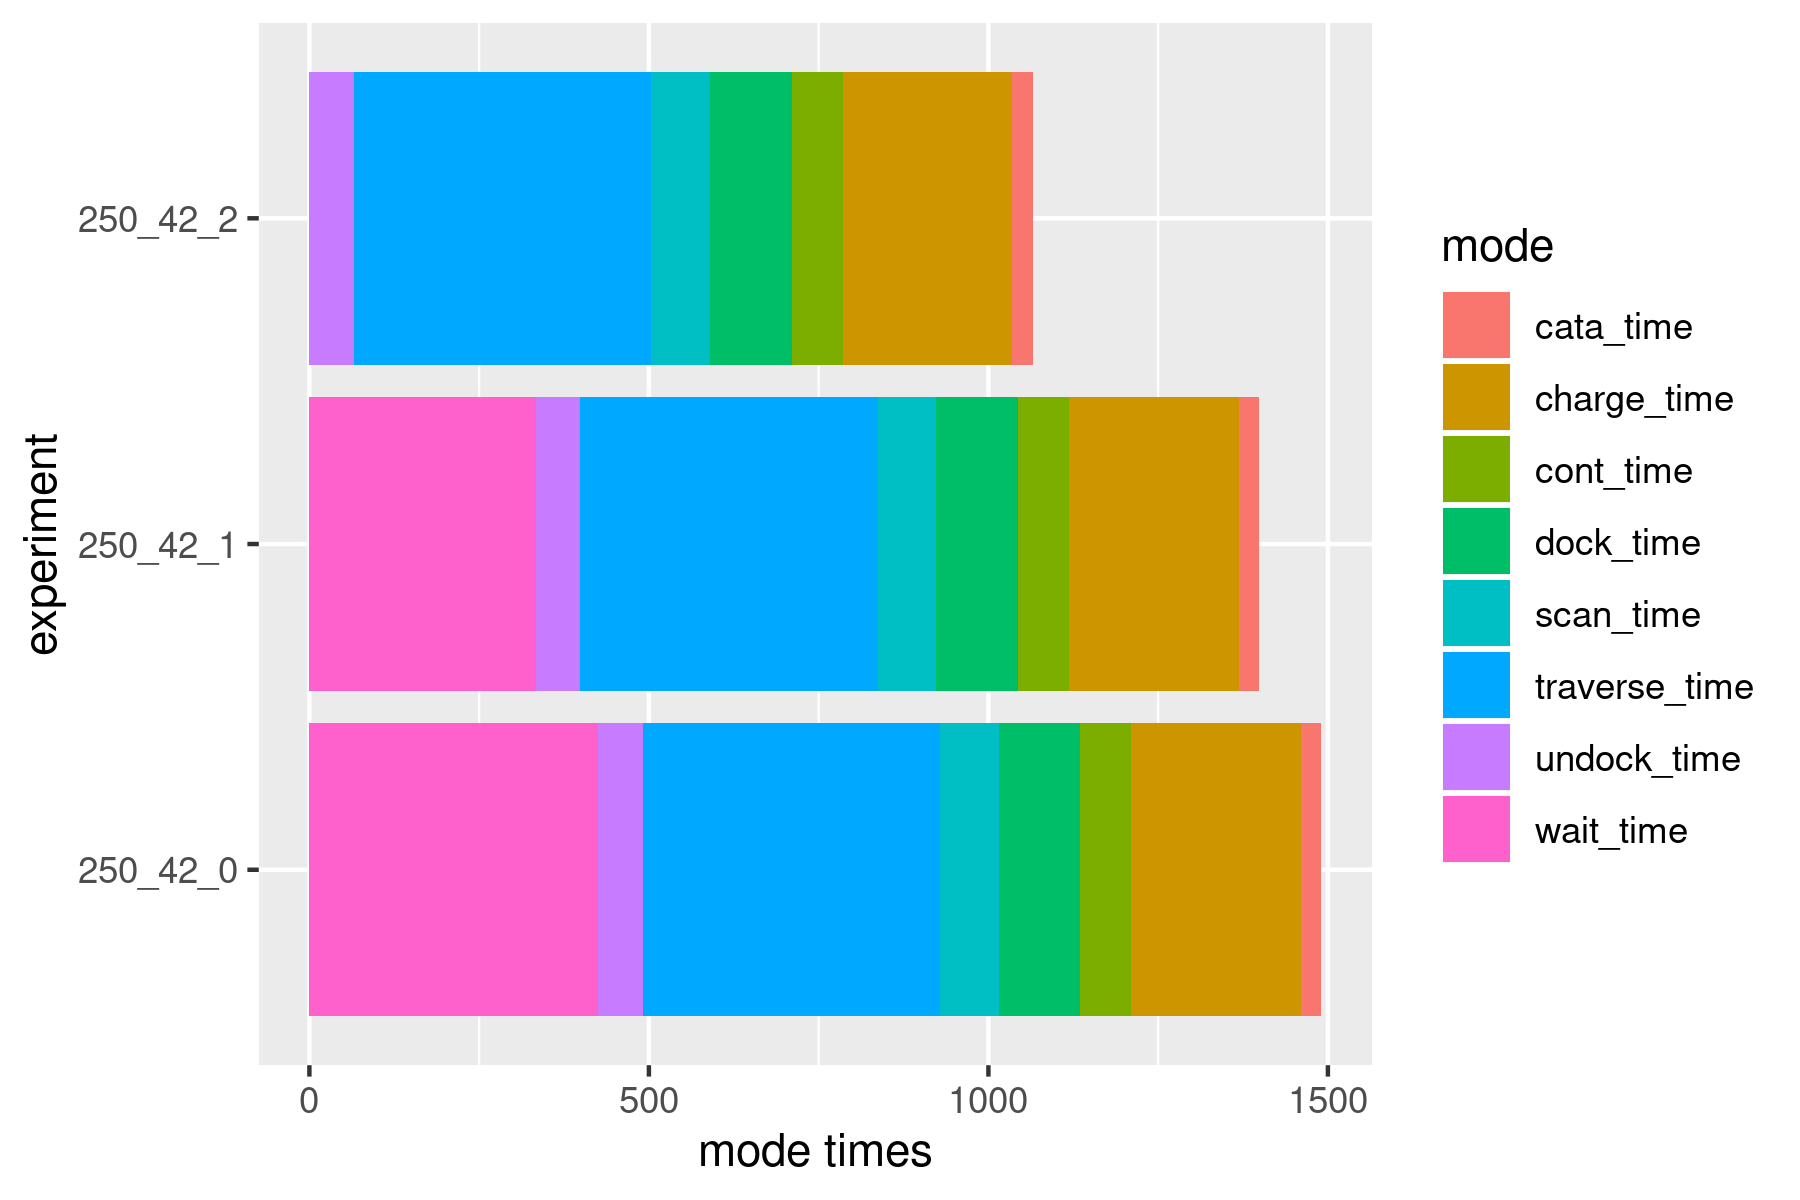
\includegraphics[width=\textwidth]{img/mode_times.png}
  \end{figure}
\end{frame}

%------------------------------------------------
\section{Fazit / Ausblick}
%------------------------------------------------

\begin{frame}
  \frametitle{Fazit}
  \begin{itemize}
    \item \textbf{Funktionalität} des integrierten Systems \textbf{demonstriert}
    \item Praktisch relevante \textbf{Probleme identifiziert und klassifiziert}
    \item \textbf{Generisches Monitoring(-Resolution)-Framework} entwickelt
    \item \textbf{Sämtliche Problemtypen in Kategorie $(1)$ / $(2)$ verschoben}
  \end{itemize}
  \textrightarrow \thinspace Erheblich \textbf{verbesserte Robustheit} bzgl. der identifizierten Herausforderungen
\end{frame}

\begin{frame}
  \frametitle{Aus Erfahrung lernen..}
  \code{mongodb\_store}
  \begin{figure}[H]
    \centering
    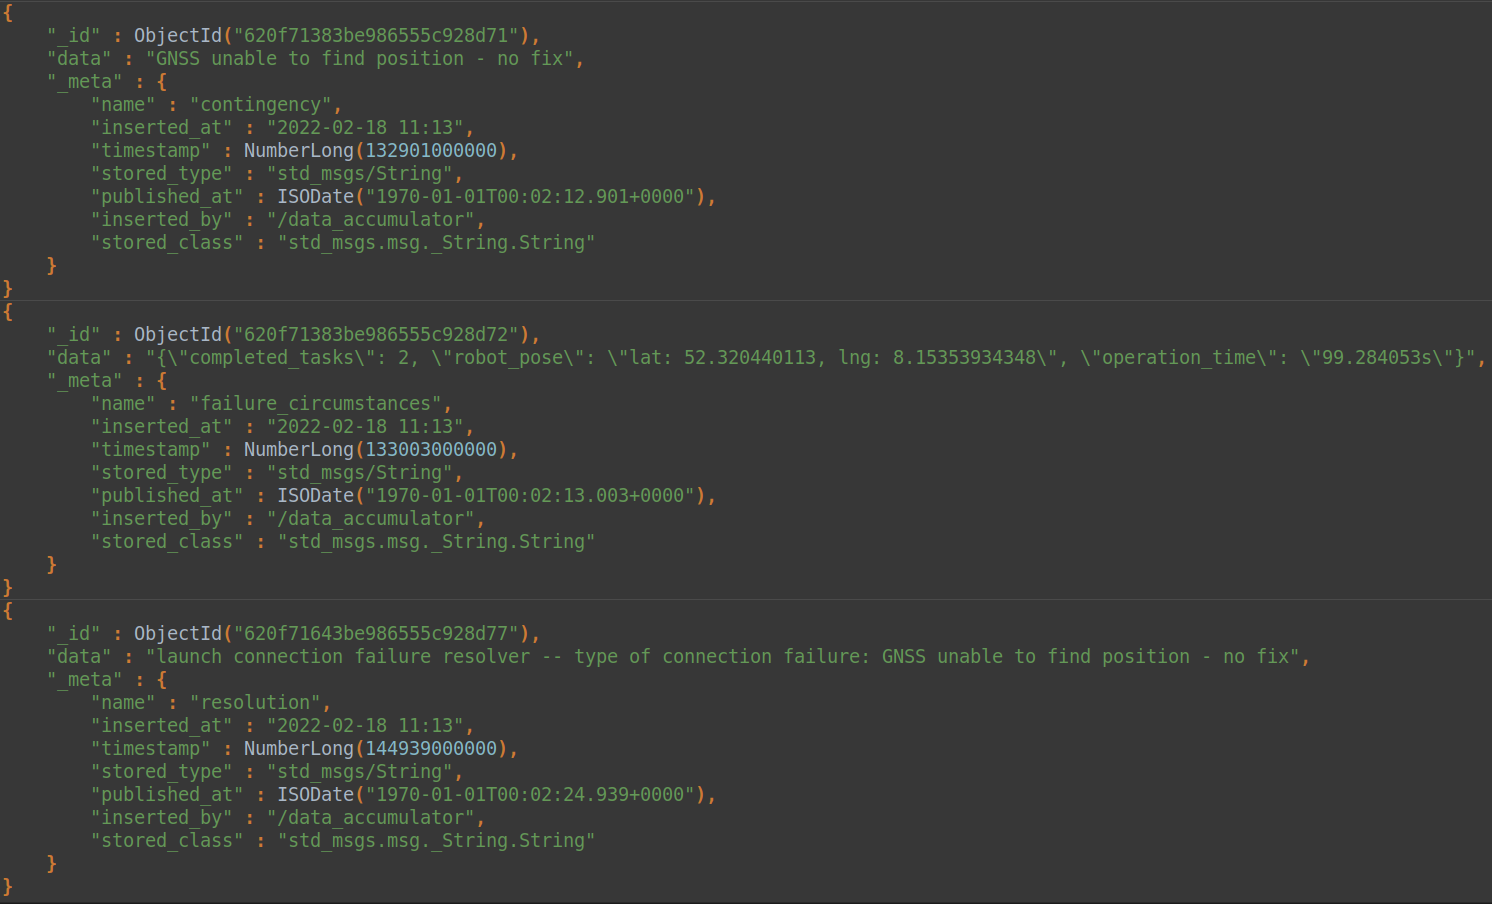
\includegraphics[width=0.8\textwidth]{img/database_entries.png}
  \end{figure}
  \begin{itemize}
    \item Ausführliche \textbf{Protokollierung der LTA-Missionen} (insbesondere Fehlerkontext)
    \item Gesammelte \textbf{Daten semantisch gruppiert}
  \end{itemize}
\end{frame}

\begin{frame}
  \frametitle{Ausblick}
  \begin{itemize}
    \item \textbf{Praxistest} mit dem AROX-System
    \item Mehr \textbf{Experimente} (Seed, Laufzeit, Fehlerfrequenz, etc.)
    \item Datenbankeinträge nutzen: \textbf{Aus LTA-Missionen lernen}
    \item \textbf{Elaboriertere Lösungsmethoden} (Fokus hier Detektion)
    \item \textbf{Web-Interface}: Remote-Zugriff auf Sensoren / Kontrolle
    \item \textbf{Usability}: Einbindung / Rekonfiguration d. Frameworks
  \end{itemize}
\end{frame}

\begin{frame}[allowframebreaks]
  \bibliographystyle{plain}
  \bibliography{sources.bib}
\end{frame}

\end{document}
